\documentclass[11pt]{report}
\usepackage[utf8]{inputenc}
\usepackage[a4paper,top=3cm,bottom=2cm,left=3cm,right=3cm,marginparwidth=1.75cm]{geometry}
\usepackage[utf8]{inputenc}
\usepackage[acronym]{glossaries}
\usepackage{tabularx}
\usepackage{graphicx}
\usepackage{listings}
\usepackage{color}
\definecolor{codegreen}{rgb}{0,0.6,0}
\definecolor{codegray}{rgb}{0.5,0.5,0.5}
\definecolor{codepurple}{rgb}{0.58,0,0.82}
\lstdefinestyle{mystyle}{
    commentstyle=\color{codegreen},
    keywordstyle=\color{magenta},
    numberstyle=\tiny\color{codegray},
    stringstyle=\color{codepurple},
    basicstyle=\scriptsize\ttfamily,
    breakatwhitespace=false,         
    breaklines=true,                 
    captionpos=b,                    
    keepspaces=true,                 
    numbers=left,
    numbersep=5pt,
    showspaces=false,                
    showstringspaces=false,
    showtabs=false,                  
    tabsize=2,
    frame=single
}
\lstset{style=mystyle,
        framextopmargin=6pt,
        framexbottommargin=6pt
        }

\graphicspath{ {images/} }
\usepackage{algorithmic}
\usepackage{hyperref}
\hypersetup{
    colorlinks,
    citecolor=black,
    filecolor=black,
    linkcolor=black,
    urlcolor=black
}

% commands for including the picture
\newcommand{\titlepicture}[2][]{%
  \renewcommand\placetitlepicture{%
    \includegraphics[#1]{#2}\par\medskip
  }%
}
\newcommand{\placetitlepicture}{} % initialization

\usepackage[style=authoryear-ibid,backend=biber]{biblatex}
\addbibresource{references.bib}

\setlength{\parindent}{4em}
\setlength{\parskip}{1em}

\title{\includegraphics[width=10cm]{mmuLogo.png}\\Efficient Detour Computation Scheme for Electric Vehicles}
\author{Cole Mansfield}
\date{May 2021}

\makeglossaries

\newacronym{ev}{EV}{Electric Vehicle}
\newacronym{evs}{EVs}{Electric Vehicles}
\newacronym{co2}{\[CO_{2}\]}{Carbon Dioxide}
\newacronym{icev}{ICEV}{Internal combustion engine vehicle}
\newacronym{mod}{MoD}{Mobility on demand}
\newacronym{soc}{SoC}{State of charge}
\newacronym{saw}{SAW}{Simple additive weighting}
\newacronym{madm}{MADM}{Multiple-attribute decision-making}
\newacronym{cs}{CS}{Charging Station}
\newacronym{css}{CSs}{Charging Stations}

\begin{document}
\pagenumbering{gobble}
\begin{titlepage}
\maketitle
\end{titlepage}

\pagenumbering{arabic}

\begin{center}
  \normalsize\textbf{Declaration}
\end{center}
No part of this project has been submitted in support of an application for any other degree or qualification at this or any other institute of learning. Apart from those parts of the project containing citations to the work of others, this project is my own unaided work. This work has been carried out in accordance with the Manchester Metropolitan University research ethics procedures, and has received ethical approval number 26136.

\noindent
Signed: Cole Mansfield
\newpage

\begin{center}
  \normalsize\textbf{Acknowledgements}
\end{center}
\newpage

\begin{center}
  \normalsize\textbf{Abstract}
\end{center}
\newpage

\tableofcontents
\newpage

\glsaddall
\printglossary[type=\acronymtype]
\newpage

\chapter{Introduction}

\newpage

\section{Background and Motivations}



\section{Report Overview}

The remaining segments of the report are structured in the following chapters:

\begin{itemize}
  \item Chapter 2: Literature Review - This chapter analyses and evaluates previous research related to the
  \item Chapter 3: Solution Design - 
  \item Chapter 4: Solution Implementation - 
  \item Chapter 5: Performance Evaluation - 
  \item Chapter 6: Conclusion - 
\end{itemize}

\newpage

\chapter{Literature Review}

\newpage

\noindent In this chapter, the rise of electric vehicles, traffic congestion and vehicle routing will be discussed and reports surrounding these topics will be investigated. Additionally, the most cutting edge research on the electric vehicle routing problem will be discussed, analysed and compared.

\section{The Rise of Electric Vehicles}

The production and purchase of electric vehicles in recent years has been growing rapidly. Passenger EV sales increased from 450,000 in 2015 to 2.1 million in 2019 \autocite{bnefEVReport}. EVs use a rechargeable battery and electric motors for propulsion. They have many advantages that are directly contributing to their rising popularity. Companies such as Tesla and Volkswagen are progressing EV technology, innovating private transport so EVs can become more accessible to the general population and aid in the fight against climate change. In 2020, Tesla became the most valuable car company globally, a great feat for EV innovation and production as they are an EV only car company.

Due to the Covid-19 pandemic in 2020, the transport industry was hit hard with lock-downs happening across the globe and more people staying at home. EVs were also greatly impacted by this issue, although they were not as harshly impacted as their counterparts, internal combustion engine vehicles(ICEV)\autocite{IEA2020CovidReport}. Despite this, the future is positive for EVs, with government policy changes and environmental concern, they look to be on an increasing trajectory. The Sustainable Development Scenario estimates that in 2030 EVs will make up 13\% of the global car fleet, increased from 1\% in 2020 \autocite{IEA2020EVReport}.  Policies set in place around the world by various governments will also be a contributing factor in the continuing rise. Seventeen countries have announced 100\% zero-emission targets as well as phasing out internal combustion engines through till 2050, with France being the first to put the intention into law \autocite{IEA2020GlobalEV}. Additionally, the EV credit system implemented in China and India's Faster Adoption and Manufacturing of EVs \autocite{bnefEVReport} show the progression and push from governments to shift towards EVs and will contribute to the rise towards them in the coming years. 

\begin{figure}[h!]
  \centering
  \includegraphics[width=0.55\linewidth]{electric-car-share-in-the-sustainable-development-scenario-2000-2030.png}
  \caption{Electric car share in the Sustainable Development Scenario \autocite{IEA2020EVReport}}
  \label{fig:1}
\end{figure}

Electric vehicles have various benefits compared to their competitors that can contribute to their popularity, the main being their environmental benefit. The burning of gasoline produces CO2, the main gas linked to climate change. Study's have found that even though in the production of EVs more carbon is produced than ICEVs over their life-cycle \autocite{hampshire2018electric}, the carbon-emitted from EVs is up to 70\% less in countries with decarbonised power generation and in 2015 they contributed to 31\% lower emissions per vehicle-kilometre compared to petrol cars\autocite{knobloch2020net}. The increasing concern over climate change is leading to the rise of EVs, their carbon-emission reducing qualities will be a major factor in the fight against it. EVs also presents a benefit to humans health in the reduction of harmful emissions, cost-efficiency and reduction of noise pollution. A study in 2016 found that when driving a Nissan Leaf(EV) instead of a Honda Civic(ICEV) over the 10-year life of the vehicle, the estimated fuel savings would be \$4130 at a time when fuel prices were at a 10-year low \autocite{malmgren2016quantifying}.

\section{Traffic Congestion}

Traffic congestion refers to the travel delay caused by interacting vehicles on roads, particularly as the volume of vehicle traffic approaches the road's capacity \autocite{litman2016smart}. It is a global issue affecting the majority of the population of the earth, mostly in urban areas. There are two main types of traffic congestion, recurring and non-recurring. Recurring congestion is "the congestion present on a normal day if nothing bad has happened on the roadway" \autocite{hallenbeck2003measurement}, such as typical rush hour traffic. Non-recurrent congestion is defined as "unexpected or unusual congestion caused by an event that was unexpected and transient relative to other similar days" \autocite{hallenbeck2003measurement}, such as accidents on the road or weather changes.

\begin{figure}[h!]
  \centering
  \includegraphics[width=0.75\linewidth]{graphRoadNetwork.PNG}
  \caption{Representation of a road network as a graph of vertices and edges}
  \label{fig:2}
\end{figure}

Despite the Covid-19 pandemic in 2020 hitting the transport market, new vehicle registrations projections are rebounding on the market. In the UK new vehicle registrations are forecast in 2022 to have increased by 30\%  from 2020 \autocite{smmtnewCars}. Traffic congestion is expected to increase with the growing vehicle population. As well as the vehicle population, the growth in the general population will increase traffic congestion. The UK population is projected to grow by 3 million by 2028 \autocite{nashnational}, meaning there will be more trips needed to be taken, equating to more congestion. Traffic from 2014 to 2019 escalated by 7.2\% \autocite{dotRoadEstimates} and through the rises in vehicle population and general population, is forecast to rise further between 17\% and 51\% by 2050 \autocite{roadtrafficforecasts}.

Both types of congestion affect people daily, adding significant delays in their lives. It has substantial economic and social impacts on society. A 2019 traffic report scorecard found that the average British driver lost 115 hours annually due to traffic congestion, and overall £5.2 billion was lost \autocite{reed2019inrix}. These can have negative factors on businesses and the economy, as it is a non-productive activity and could be a direct cause for employee punctuality. Traffic congestion can also affect peoples health. Stress and aggressiveness brought on through traffic congestion can be detrimental to others safety on the roads and cause more delays. The 2019 RAC Report on Motoring found that increasing traffic levels is the most common cause of stress at 40\%, which represents 10 million motorists \autocite{racreportonmotoring}. The congestion issue is of significance and if not managed, will continue to disrupt different parts of society. 

\section{Vehicle Routing}

\subsection{Overview}

Vehicle routing is one of the main ways of combating traffic congestion. Finding the optimal shortest path between two vertices in a network of vertices is a challenging task studied in graph theory. When applying this concept for vehicle routing we would present the vertices and edges as systems of junctions and roads. When adding vehicles into the problem it becomes more problematic due to weather conditions, traffic congestion and the state of the road. Choosing the correct algorithm is a problem for many current transportation navigation systems, there are numerous approaches developed to tackle this issue, each with its pros and cons.

Optimal based shortest path algorithms guarantee to find the optimal solution through exploring the whole set of available solutions \autocite{nha2012comparative}. One example of an optimal based algorithm is Dijkstra. Dijkstra is one of the most used shortest path algorithms \autocite{broumi2016applying}, created in 1959 by Edsger W. Dijkstra. It finds the shortest path between two nodes in a graph \autocite{dijkstra1959note}. The route is found by initially creating a set of nodes not visited, then beginning at the starting node and calculating the cost of movement to each node connected to the starting node \autocite{pathComparison2012}. After all neighbouring nodes have been considered, the starting node is then deleted from the nodes not visited set and the next node is chosen as the one with the lowest cost of movement from the starting node \autocite{pathComparison2012}. These steps are then iterated until the destination node is deleted from the nodes not visited set or all nodes have been considered \autocite{pathComparison2012}.

Heuristic-based shortest path algorithms explore available solutions and find an approximate optimal solution that is close to or the same as the optimal one \autocite{nha2012comparative}. The main heuristic-based approach developed is the A* algorithm \autocite{hartAStar}. Created in 1968 by Peter E. Hart, Nils J. Nilsson and Bertram Raphael, it is seen as an extension of Dijkstra but a more general approach to the shortest path problem \autocite{pathComparison2012}. The difference between the two is that A* introduces a heuristic in which nodes are chosen when searching for the route. A heuristic is a function that is used to solve problems faster and when traditional problems fail to find a solution. In the case of A*, the most popular method used for the heuristic calculates the distance from the node currently being evaluated to the end node, then using that cost in the decision of which node to go to next.

In addition to A* another example of a heuristic-based approach is the genetic algorithm \autocite{haupt2004practical}. It is a meta-heuristic used to solve optimisation problems and is based on the principles of genetics and natural selection \autocite{bagheri2008finding}\autocite{nha2012comparative}. The genetic algorithm has been used in the shortest path problem and can be an approach to solving harder problems that come about such as when vehicles have to visit all nodes in a large network \autocite{genAlgs1997}.

The different algorithms for the shortest path problem have advantages that better suit them for specific scenarios. Heuristic-based approaches reduce computation time but can be more resource dependant due to more memory usage for storing the heuristic. Dijkstra and A* will always give the best route solution as long as A* does not overestimate the heuristic \autocite{wang2013comprehensive}. Meta-heuristic optimisation approaches such as genetic algorithm and tabu search are better suited for multi-location vehicle routing, where the data set is much larger.

\subsection{Electric Vehicle Routing}

When it comes to routing electric vehicles the problem becomes more difficult. Extra constraints when routing EVs make calculating a route more challenging than normal ICEVs do. Firstly, EV charging station infrastructure is still not there, with demand for chargers rising rapidly. The UK would need to install charging stations five times faster if it was to reach between 300,000 and 500,000 stations, which is required for 2030 with current EV projections \autocite{charginUpPolicyExchange}. Refuelling times of EVs is also a problem that needs to be factored in when routing. An EV can take between 26 hours for the slowest chargers (alternating current chargers) and 6 minutes for the fastest chargers (direct current fast chargers) to add 100 miles to its range \autocite{lee2018charging}. With the charging station infrastructure not being there and the added issue of timely charging, the availability of them is also affected. With EV demand and consumption continually growing and government policy changes around the globe, the issue will only worsen without major changes. Range anxiety is a concern of EV drivers, the fear of battery capacity depleting mid-trip \autocite{neubauer2014impact}. This is something that could be reduced with electric vehicle routing and progression in charging station infrastructure. Additionally, conditions in the EVs environment can affect battery capacity such as the weather. A 2019 study found that an EV at 20°F resulted in a 12\% decrease in driving range and when the HVAC (Heating, Ventilation and Air Conditioning) system was used there was a 41\% decrease. This could result in a need for more charges and will put a strain on charging station availability at colder temperatures \autocite{aaaEVWeather}. With these added constraints a new comprehensive solution for electric vehicle routing needs to be developed to reduce range anxiety in EV users.

\section{Related works}

\subsection{Route Search Method for Electric Vehicles in Consideration of Range and Locations of Charging Stations \autocite{kobayashi2011route}}

Researchers at the Yokohama Research Laboratory in Japan proposed this paper introducing a new routing search solution for EVs. Their proposal investigated how to calculate a route for EVs based on stops at charging stations if the current battery capacity was not enough to reach the destination, providing a route with the minimum travelling cost.

Their method takes the EV range and charging stations locations, and calculates through the range a new route. When the current range of the EV is sufficient enough to reach the destination without the need for a refuelling stop, a route is calculated conventionally with the remaining capacity on arrival. Meanwhile, when the starting range is insufficient, charging stations based on the EVs range are selected as potential stops. Then with the distance between charging stations, estimated travel time and estimated charging time, the most cost-effective route is selected. Routes were created based on Dijkstra's algorithm and the appropriate charging stations. The algorithm was then evaluated on a Japanese map with hypothetical charging stations on the route, assessing execution time for selecting potential charging stations and for conventional route searching with some of the selected charging stations. 

\begin{table}[h!]
\begin{center}
\begin{tabular}{|p{0.3cm} p{2.2cm} p{2.2cm} p{1.3cm} p{1.3cm} p{0.5cm} p{1.3cm} p{1.3cm} p{1.3cm}|} 
 \hline
 No & Departure Point & Destination & Travel distance & Travel Time & \# SCS & POI Search Time & Route Search Time  & Total Search Time \\
 \hline
 1 & Narita Airport & Maihama station & 62.784 & 1.542 & 1 & 3.46 & 7.06 & 10.52\\ 
 2 & Narita Airport & Maihama station & 58.434 & 0.874 & 0 & 2.71 & 5.63 & 8.34\\
 3 & Narita Airport & Maihama station & 58.434 & 0.874 & 0 & 2.78 & 5.63 & 8.41\\
 4 & Narita Airport & Hachioji Station & 121.941 & 3.033 & 2 & 6.40 & 13.41 & 19.81\\
 5 & Narita Airport & Hachioji Station & 112.772 & 2.303 & 1 & 6.41 & 16.20 & 22.61\\
 6 & Narita Airport & Hachioji Station & 109.548 & 1.652 & 0 & 4.24 & 9.09 & 13.33\\
 7 & Narita Airport & Atami Station & 200.522 & 4.953 & 2 & 6.01 & 16.98 & 22.99\\
 8 & Narita Airport & Atami Station & 200.522 & 4.786 & 2 & 6.29 & 16.98 & 23.27\\
 9 & Narita Airport & Atami Station & 167 953 & 3 834 & 1 & 6.74 & 13 98 & 20.72\\
 \hline
\end{tabular}
\end{center}
\caption{Simulation results \autocite{kobayashi2011route}}
\label{table:1}
\end{table}

The results in Table \ref{table:1} shows that the Point of Interest search time, which is the execution time for selecting charging stations and the route search time, was evidently higher for users needing to stop at charging stations. The computation time can be seen as much faster and more accurate than manually planning CS visits on the route. Also, their solution computes routes with accessible charging over a large network efficiently. A drawback of the solution is its failure to evaluate charging stations further. Checking the availability and current capacity of charging stations are things that could affect journey times and distances needing to be travelled. Additionally, it does not take into account time delays such as traffic when evaluating routes.

\subsection{A Bellman-Ford approach to energy-efficient routing of electric vehicles \autocite{bellmanFordRouting}}

This paper from researchers at Oakland University presents a routing solution for electric vehicles focusing on energy efficiency. They model an electric vehicle with accurate energy consumption and then find the optimal route using a bellman-ford approach. They aim to tackle the energy-efficient routing problem in its most simple form.

The researchers first present an EV model and calculate vehicle power output using parameters such as vehicle mass, gravitational acceleration, tire rolling resistance coefficient, mass density and drag coefficient. They also calculate the regenerative braking power of the vehicle and net energy consumption. Using this model they compute the route from the start to the destination through the graph using the bellman-ford algorithm, finding the energy consumption between each node and making decisions on which path to take based on the least energy consumption from node to node. The bellman-ford algorithm \autocite{bellman1958routing} is a similar pathfinding algorithm to Dijkstra although its main difference is its capability to find a path even with negative edge weightings. It is used in this solution due to the possibility of node to node energy consumption being negative.

Their proposal was then simulated on various map sizes represented as graphs. From this, they found in large scale maps that their approach cannot be used for routing and is impractical, with path generation taking 203 hours on a graph with 270,780 edges. Although on smaller-scale maps it is effective with it taking 0.128 seconds on a graph with 63 edges. Their solution is adequate and finds routes based on energy efficiency for EVs in small networks with bellman ford working well for energy weighted graphs. Also, the EV energy model is an accurate representation of EV energy consumption. A downside of the model is its failure to highlight environmental issues such as the impact of weather conditions on the battery consumption speed. Another limitation to the routing proposal is that it does not take into account charging and charging station selection when routing. As an extension to this solution, traffic conditions and vehicle remaining range could be taken when computing routing decision. 

\subsection{Optimal Routing with In-Route Charging of Mobility-on-Demand Electric Vehicles  \autocite{inRouteOptimalAmmous}}

This work from the University of Idaho in the USA develops a routing solution for mobility on demand(MoD) EV systems. MoD is a one-way vehicle sharing system and is a promising way to reduce greenhouse gas emissions and a sustainable way for private mobility over the current reliance on a personal vehicle. They aim to reduce the inconvenience surrounding MoD systems with the occasional customer needing to perform in route charging and getting the optimal average trip time.

The authors propose a system of routing between multiple passenger stations while considering in-route charging and allocating passengers with fewer delay constraints to EVs needing to be charged. Using a multi-server, cloud-based infrastructure for connectivity through all components in the system, they calculate the routing probabilities of EVs to charging stations and then make routing decisions based on these. There model only considers EVs that need to be charged on the way to their destination. Their model is then simulated extensively using battery-swapping to reduce excess charging delays and different systems parameters, then evaluated against conventional shortest time decisions.

The results from the simulations carried out show a reduction in charging station delays and trip times compared to other shortest time and random routing schemes. MoD systems could be a great implementation for private mobility using electric vehicles and be a future system of transport to tackle population growth and climate change. The presented solution for routing and scheduling of vehicles in the system finds optimal solutions and would significantly reduce frustration levels of customers that are forced to charge in-route.

\subsection{Implementation of charging station based electric vehicle routing problem using nearest neighbour search algorithm  \autocite{csNearestNeighbourDaanish}}

This paper from the Indian Institute of Technology proposes a nearest neighbour approach to EV routing, finding the most energy-efficient route. This work aims to develop a new routing solution for EVs taking into account vehicle battery capacity and charging stations after the recent surge in EV market share and the environmental benefits they bring with them.

Their solution concentrates on multi-node traversal where each node only can be visited once. Using Dijkstra's algorithm from each current node they find the next nearest node in the graph. They iteratively do this until each node has been visited once. For routing an EV, their solution checks whether the vehicle can make it to the next node or next charging station without losing all charge, charging fully at each charging station it visits, and again iteratively checking at each node whether the vehicle will make the journey to the nearest neighbour. This was then simulated using coordinates of cities(nodes), finding the accurate optimal solution based on the shortest route between each city.

The simulations results revealed accuracy when calculating an optimum routing path for EVs with charging taken into account. It also showed a good basic solution to multi-stop vehicle routing, with checks on vehicle current range and routing the vehicle via charging stations when current battery capacity could not reach the next city(node). As an extension, the algorithm could have a better estimation of EV range to take in more vehicle parameters such as vehicle weight, front Surface area and propulsion efficiency. Also, route constraints such as traffic and weather conditions could be incorporated into the algorithm to test its effectiveness against real-world scenarios. Furthermore, accessing the algorithm next time against more conventional routing solutions would give a better insight into how well it performs.

\subsection{Distributed Routing and Charging Scheduling Optimisation for Internet of Electric Vehicles  \autocite{distributedRoutingTang}}

Work by researchers at the Chinese University of Hong Kong developed a routing and charging algorithm for an internet of electric vehicles(IoEV). Their solution allows routing to be calculated in a distributed manner by users and a system operator. They aim to protect the anonymity of users and reduce the computational complexity of the system operator. Their algorithm selects an approximate path for each EV, then optimises the charging scheduling of the EVs based on the approximate path. This was then simulated extensively, comparing it with two other benchmark algorithms on a dataset that maps real-world data to nodes and edges from Washington D.C.

Overall the simulation results showed that the proposed routing solution outperformed the two conventional methods used in the simulation and that it always produced a near-optimal performance with low computational complexity. Using an IoEV is a promising way of tackling the NP-hardness and computational complexity of EV routing for larger systems with multiple destinations, such as delivery couriering. Having a centralised location for distributing EVs and scheduling them at charging stations would also reduce queuing times at charging stations and allow for improved selection. A downside of their proposal is the infrastructure needed to be put into place to get the system up and running, needing a centralised system to manage multi-car rerouting. To extend their implementation, we propose to incorporate charging station availability into decision making which could further decrease travel and wait times.

\subsection{Electric Vehicle Charging Warning and Path Planning Method Based on Spark \autocite{sparkEVChargingDing}}

Researches from the Xi’an University of Technology in China propose a shortest time path planning algorithm with an energy consumption warning method for EVs with an insufficient battery capacity for their journey. They also use the java Spark Parallelization framework \autocite{spark} to reduce computation time. It was designed to help EV drivers with the charging problem of slow charging times, small charging station availability and best charging station to route to.

They first present an energy warning model which monitors the energy consumption of the vehicle and using its average speed and regression coefficients, issues a warning when the current battery capacity of the EV will not reach its destination. Then a path planning algorithm is developed. They use Dijkstra's algorithm to find the shortest path from the current node to charging stations and the destination, choosing the optimal charging station to stop factoring in queuing and charging times. When calculating the shortest path they also implemented Spark to compute the shortest path in parallel to improve the efficiency of the algorithm. Their solution is then run through a real-world traffic network to test its effectiveness.

Simulation results showed with the addition of Spark to run Dijkstra computations at the same time, it had a significant reduction in the time taken to find the optimal route. Notably when the number of nodes in the graph grew larger the run time of the algorithm dropped compared to small graphs, for example on a road network with 300 nodes the computation time decreased from 1.2s to 0.1s. The implementation of synchronous computing in the routing algorithm is an encouraging feature for large pathfinding in networks.

\subsection{Optimization of Electric Vehicle Routing Problem Using Tabu Search \autocite{optimizationTabuSearch}}

This work from Northeastern University in China presents a pathfinding solution to the electric vehicle routing problem(EVRP). They use the Tabu Search approach to multi-objective route planning for EVs and aim to combat the issues of limited battery capacity and charging demands when routing these vehicles. They aim to optimize routing for logistics services when using EVs as the issue becomes more prominent with major US companies implementing fleets of these vehicles.

The authors propose a routing solution using Tabu search, where the vehicle has multiple destinations to visit on their journey. Tabu search is an optimization technique that uses a meta-heuristic and Tabu list in which mimics the human memory function, blocking all areas that have been searched in a route to avoid detours. It begins by creating a random initial route, then from that searches for possible routes, comparing each route until it finds the optimal one, taking into account electrical charging demands of the EVs. Their proposal is then evaluated using coordinates of locations, charging stations and the locations needed to be visited.

\begin{table}[h!]
\begin{center}
\begin{tabular}{|p{3cm} p{3cm} p{3cm} p{3cm}|} 
 \hline
 Method & Node Number & Result(km) & Time(s) \\
 \hline
 Tabu Search & 20 & 247 & 5s \\ 
 & 30 & 422.56 & 5s \\
 CPLEX & 20 & 247 & 49s \\
  & 30 & 422.56 & 358s \\
 \hline
\end{tabular}
\end{center}
\caption{Tabu search results comparison \autocite{optimizationTabuSearch}}
\label{table:2}
\end{table}

The Tabu search solution was then evaluated against another commercial routing algorithm and the results are shown in Table \ref{table:2}. They show routing for two different distances and how the time taken for Tabu search was significantly reduced, with no time increasing with distance increase, unlike the CPLEX. Overall the proposed algorithm is a good solution to the routing problem using EVs with multiple stops. It has significant time reductions on other existing solutions and always finds the optimal route considering EV battery limitations. An improvement of their proposal would be to add in better choosing of CSs, taking into account availability and efficiency. Also extending their evaluation to examine their proposed solutions performance on destination to destination routing and assessing it against a few more routing algorithms would allow us to have a better understanding of the true overall performance of their routing solution. 

\section{Comparative Study}

Each of the related works aims to design a routing solution for electric vehicles and tackle the new associated issues. To begin it is clear that all charging station constraints need to be taken into account when deciding on which to route via. The path planning method proposed by researchers at the Xi’an University of Technology \autocite{sparkEVChargingDing} considers more charging station constraints, such as vehicles waiting and charging times when making a decision, making the path calculated more optimal for an EV. Compared to earlier works, such as \autocite{kobayashi2011route} and \autocite{bellmanFordRouting}, where these constraints were not considered, this work allows for better judgement on the true optimal route. Moreover, the mobile on-demand proposal includes a promising idea with charging station schedule, although this would, in turn, affect the privacy of drivers and their vehicles \autocite{inRouteOptimalAmmous}. To further include the above works, the inclusion of more constraints for charging stations such as CS charging efficiency, price and vehicles waiting will ensure better accuracy in the computing of the optimal route.

Below is table \ref{table:4} that illustrates related works and highlights how important components have been implemented.

\begin{table}[h!]
\begin{center}
\begin{tabular}{|p{3cm} p{2.8cm} p{2.8cm} p{3cm} p{3cm}|} 
 \hline
 \bf{Study} & Complexity & CS Attributes & Scalability & Overall Effectiveness \\
 \hline
 \bf{\autocite{kobayashi2011route}} &  &  &  & \\ 
 \bf{\autocite{bellmanFordRouting}} &  &  &  & \\
 \bf{\autocite{inRouteOptimalAmmous}} &  &  &  & \\
 \bf{\autocite{csNearestNeighbourDaanish}} &  &  &  & \\
 \bf{\autocite{distributedRoutingTang}} &  &  &  & \\
 \bf{\autocite{sparkEVChargingDing}} &  &  &  & \\
 \bf{\autocite{optimizationTabuSearch}} &  &  &  & \\
 \hline
\end{tabular}
\end{center}
\caption{Comparative Study table}
\label{table:4}
\end{table}


\section{Conclusion}

To conclude, the research in this chapter shows the growth of electric vehicles and the upwards trajectory they are on. Also, the significant effects of traffic congestion, the problems that come with it and the vehicle routing that can be used to reduce it. Then, the issue of routing electric vehicles and the research done to combat this was investigated. On investigation of the related works, it is evident all charging station constraints need to be considered when making a decision on which one to route through. In addition, all vehicle parameters need to be taken into account when estimating vehicle range, to ensure correct charging station selection is done based on the current EV range and accurate decision regarding the need for charging.

\newpage

\chapter{Solution Design}

\newpage

\noindent This chapter provides an overview of the proposed routing algorithm, including routing algorithm chosen and charging station selection. In addition, the tools needed and software development methodology followed throughout the project will be presented.

\section{Routing Process Design}

The detour routing algorithm will attempt to find the optimal route for an EV taking into account current vehicle range, route length and traffic. Figure \ref{fig:3} below shows a high-level overview of the algorithm as a flowchart.

\begin{figure}[h!]
  \centering
  \includegraphics[width=0.56\linewidth]{AlgFlow.png}
  \caption{Flowchart of the algorithm}
  \label{fig:3}
\end{figure}

Finding a detour will be initialised when the current location of the EV and the destination is inputted. A route is then calculated from these two points using the path searching technique described in Section 3.2. When evaluating each node, stopping criteria is put in place that checks whether the current EV range is sufficient enough for the current route length and ensures that it does not fall below the minimum SoC(state of charge), which is defaulted at 10\%. Having this stopping criterion will reduce computation time as calculating the full route is unnecessary due to inadequate battery capacity. 

If the route reaches the end node without dropping below the minimum SoC then the route is outputted back to the user. When it falls below minimum SoC then re-routing via a charging station is initialized. A charging station is selected using the logic in Section 3.3 then a route from the start to the charging station is found again using the path search technique from Section 3.2. Once the route is found a new start point will be set after the CS location and the algorithm iterates again from the beginning with the new start point until the end is reached.

\section{Vehicle Routing Algorithms}

For the proposed solution a graph traversal algorithm is needed to calculate optimal routes for vehicles. There are numerous methods developed for computing how a vehicle will traverse a network, starting at one designated point and ending at another. As discussed in the literature review, there are algorithms developed in graph theory that searches for a path in the graph, typically the shortest one. Numerous popular algorithms were considered to be used when finding the path such as Dijkstra, A*, Tabu search, genetic algorithm and Breadth-first traversal. The main aims of the algorithm are for it to find the optimal route, faster computing times and the ability to incorporate more constraints than distance such as travel time when routing.

\subsection{Chosen Path Search Algorithm}

On the evaluation of the algorithms used for graph traversal and vehicle routing, the A* algorithm is the one being used to traverse the vehicle network and find an optimal route. As mentioned above in the literature A* is a heuristic-based pathfinding algorithm that is considered an extension of Dijkstra. 

A* was the chosen algorithm due to various factors. Firstly, the use of a heuristic function benefits the solution. The main benefit being faster computation times due to searching fewer nodes, which is also beneficial when the number of nodes in a graph increases. In addition, when the heuristic is admissible (can never overestimate the cost to reach the goal) A* is guaranteed to output the optimal path which has the least cost \autocite{rana2011star}. Additionally, the complexity of A* compared to the meta-heuristic techniques, such as Tabu search and genetic algorithm, is a lot lower, making it easier to implement and add custom constraints. Likewise, these techniques are better suited for multi-objective routing problems such as the vehicle routing problem and travelling salesman problems where routing criteria and graph size is much larger. 

\begin{figure}[h!]
  \centering
  \includegraphics[width=0.78\linewidth]{a-star.png}
  \caption{A* pseudo-code \autocite{cox_2020}}
  \label{fig:4}
\end{figure}

\subsection{Network Costs and Heuristic}

Equation \ref{eq:1} shows the A* path cost formula which uses the minimum value for path selection.
\begin{equation} \label{eq:1}
f(n)=g(n)+h(n)
\end{equation}
The term denoted as \emph{g(n)} traditionally is the cost of movement from the start node to the current node(n) in the graph (the weight from node to node in the network). The term \emph{h(n)} is traditionally the heuristic function which estimates the cost of movement from the current node to the destination node. \emph{h(n)} is usually calculated through a euclidean distance which is denoted in the equation \ref{eq:2}, with p and q being coordinates of nodes in the graph \autocite{pathComparison2012}.
\begin{equation} \label{eq:2}
 d\left( p,q\right)   = \sqrt {\sum _{i=1}^{n}  \left( q_{i}-p_{i}\right)^2 } 
\end{equation}
When finding a path for vehicle routing, using the traditional methods for A* will not suffice because typically more real-world constraints such as traffic affect routing choices and finding the shortest path will only find the optimal shortest solution. Instead, our goal is to minimize the travel time of a vehicle routing, changing the traditional cost values for \emph{g(n)} and the heuristic function \emph{h(n)} from equation \ref{eq:1} to fit this criterion.
\begin{equation} \label{eq:3}
    g(n)=l(n)/s(n)
\end{equation}
\begin{equation} \label{eq:4}
    h(n)=d(n)/m(n)
\end{equation}
Equation \ref{eq:3} denotes the new value of \emph{g(n)}, which is the travel time from the start node to the current node(n) in the graph. This is calculated by dividing the length from the start node to the current node which is shown as \emph{l(n)} by the last time steps mean edge speed for the same nodes, which is denoted as \emph{s(n)}. Equation \ref{eq:4} denotes the new heuristic function formula for the value \emph{h(n)}. \emph{d(n)} represents the Euclidean distance calculation used in the traditional A* heuristic function, this is then divided by \emph{m(n)} which is the max speed of any edge in the network. Using the max speed of any edge in the network allows us to never overestimate the cost to reach the goal for the heuristic, which makes it admissible and gives us the optimal route.

\section{Charging Station Selection}

Selection of the optimal charging station is needed for the optimal solution. Figure \ref{fig:5} depicts a visual representation of charging station selection from the search node. Various parameters are needed to be taken into account when making a decision on which charging station the vehicle should refuel at, making it a multiple-attribute decision-making (MADM) problem. There are numerous methods developed to help make optimal decisions and the technique we will use is simple additive weighting (SAW). Selection begins by getting all CSs in range of EV current battery capacity and then makes a decision on the best with the SAW method. The centre point of the range is first defined as the node from where the initial route calculation dropped below the minimum SoC and if no CSs found from there, the node changes to the starting point if the search node is not initially that.

\begin{figure}[h!]
  \centering
  \includegraphics[width=0.85\linewidth]{CSSelection.png}
  \caption{Visual representation of charging station selection}
  \label{fig:5}
\end{figure}

\subsection{Simple Additive Weighting (SAW)}

SAW is one of the most popular and best-known MADM techniques used \autocite{chakraborty2007simulation}. It uses a weighted sum of all attributes for each instance of objects and compares the total of each, with the higher overall weighted sum being the better choice \autocite{churchman1954approximate}. 

To begin, each attribute value needs to be normalised for each charging station, making each value within a common scale so values with more extreme ranges do not influence the end summation. There are many different techniques for data normalization such as linear, min-max, vector and logarithmic normalization. A 2007 comparative study on normalization procedures in MADM found that vector normalization is the most suitable for SAW \autocite{chakraborty2007simulation}.
\begin{equation} \label{eq:5}
    r_{ij} = \frac{x_{ij}}{\sqrt{\sum_{i=1}^{m}x_{ij}^{2}}}
\end{equation}
\begin{equation} \label{eq:6}
    r_{ij} = 1 - \frac{x_{ij}}{\sqrt{\sum_{i=1}^{m}x_{ij}^{2}}}
\end{equation}
Equation \ref{eq:5} shows the formula used to normalize the data using beneficial vector normalization and equation \ref{eq:6} shows non-beneficial vector normalization. The beneficial formula is used when the attribute's value aims to be higher and the non-beneficial used when the value desired is lower. Once the data has been normalized each value can then be multiplied by their weighting value. 
\begin{equation} \label{eq:7}
    v_{i}=\sum_{j=1}^{n} w_{j} \cdot r_{ij}
\end{equation}
Weightings are determined by how much the given parameter matters when making a decision and all have to add up to 100\%. Equation \ref{eq:7} depicts the calculation that gets the score for each charging station based on SAW. \emph{i} is the index of the charging station, \emph{v}
is the overall score and \emph{j} is index of the CS parameter. \emph{r} holds the added score of the CS parameters and \emph{w} is the weighting value for the given parameter. Parameters for each charging station is multiplied by its weighting then each summed together for its overall score.

\subsection{Charging Station Decision Attributes}

Deciding on which CS to route via requires the decision attributes to be defined. Table \ref{table:3} illustrates the parameters used in SAW. The distance from the start is the straight line distance from the current node to the CS. Distance from divider is the straight line distance from a line that connects the current node and end node, this highlights whether the CS is in the right direction. Figure \ref{fig:5} shows visually how the distances work in context with the charging stations in the vicinity of the EV current range. Refuelling price, the number of vehicles charging and charging efficiency are CS properties. Charging efficiency is the KW gained by EV battery per time step from the CS.

\begin{table}[h!]
\begin{center}
\begin{tabular}{|p{6cm} p{3cm}|} 
 \hline
 Attribute Name & Normalization \\
 \hline
 Distance From Start & Non-beneficial  \\ 
 Distance From Divider & Non-beneficial  \\ 
 Price & Non-beneficial  \\ 
 Vehicles Charging & Non-beneficial  \\ 
 Charge Per Step & Beneficial  \\ 
 \hline
\end{tabular}
\end{center}
\caption{Charging station attributes for SAW MADM}
\label{table:3}
\end{table}

\section{Development Methodology}

An agile approach was the software development methodology used throughout the project. Agile is a popular and industry-leading methodology that uses an iterative approach to software development project management. Project requirements are split and each stage is set out. Iterations are done for each requirement split until each stage has been complete for that section. It is a well ordered and structured methodology that creates adjustability and adaptation \autocite{InsightstoAgile}. Figure \ref{fig:6} depicts the key stages and cycle of an agile iteration.

\begin{figure}[h!]
  \centering
  \includegraphics[width=0.65\linewidth]{agileWheel.jpg}
  \caption{Agile methodology \autocite{InsightstoAgile}}
  \label{fig:6}
\end{figure}

In 2001, a group of software developers met to find common ground and came up with the agile manifesto that highlights the key values and principles \autocite{beck2001agile}. The main was:
\begin{itemize}
  \item Working, valuable software early
  \item Welcome change
  \item Working software is the primary measure of progress
  \item Sustainable development - should be able to maintain a constant pace indefinitely
\end{itemize}

Agile is the methodology being applied in the project due to its lenient and flexible working model. As well as this, it promotes constant improvement and refinement, with the project having defined aims but freedom on ways to solve the problem it is best suited.

\section{Solution Resources}

\subsection{SUMO}

The EV detour routing solution will depend upon a piece of software called \emph{SUMO}. \emph{SUMO} is an open-source microscopic traffic simulation suite that allows us to create models of road networks, simulate vehicles, pedestrians and public transport on said networks and manage each vehicle dynamically \autocite{SUMO2018}. It provides the tools needed to implement and evaluate our proposed algorithm in real-world scenarios and get an artificial real-world representation of its performance. In 2014, mathematical energy and charging models for EVs were implemented into \emph{SUMO} that mimics an EVs energy consumption and charging \autocite{kurczveil2013implementation}, which provides the ability for our EV routing solution to be simulated within \emph{SUMO}. The \emph{sumo-cli} and \emph{sumo-gui} tools give us a command-line based and graphical representation of the road networks, with time step based performance XML outputs for each vehicle. In addition, \emph{netedit} is a visual editing tool that allows us to create and edit road networks.

\subsection{Python and TraCi}

The algorithm will be implemented using the \emph{Python} programming language with the \emph{TraCi}(Traffic Control Interface) library \autocite{van1991python} \autocite{traciPython}. \emph{TraCi} is an application protocol interface(API) that allows us to receive data from the \emph{SUMO} simulator as it runs and manipulate the behaviour of objects in the simulation. \emph{TraCi} has been developed for multiple programming languages. \emph{Python} was the one selected due to its support for all \emph{TraCi} commands unlike the other implementations and its daily testing and usage. \emph{TraCi} will allow us to get current electric vehicle parameters such as battery capacity and re-route the vehicle with the computed detour from the algorithm with stops at charging stations.

\subsection{Open Street Map}

OSM(Open Street Map) is a free and editable map. With osm, it has the ability to import real-world areas into the netedit tool, randomly generate vehicle trips and public transport networks and run them using \emph{SUMO}. This will be used to evaluate the performance of the proposed detour routing algorithm in real-world scenarios.

\section{Conclusion}

To conclude this chapter outlines the overall design and techniques used for the EV detour routing algorithm. Taking into consideration research done in the previous chapter, it identified the technical requirements and the design choices made for the solution, allowing for a reduction in time on implementation. Furthermore, the development methodology followed and the resources needed were presented.

\newpage

\chapter{Solution Implementation}

\newpage

\noindent The following chapter exhibits the implementation of the proposed solution using tools and design stated in Chapter 3. Implementation is split into two main phases, \emph{SUMO} configuration and algorithm implementation. Firstly, this deals with the set-up of the simulation and the rerouting algorithm to be implemented within it. Next, the algorithm will be implemented, computing a new detour based on current EV attributes.

\section{SUMO Configuration}

\subsection{Network Building}

As mentioned in the above chapter, \emph{SUMO} will be used to simulate and evaluate the solution. \emph{SUMO} software requires artificial networks to be built to simulate intermodal traffic systems. Using the \emph{netedit} tool that is included in the \emph{SUMO} software package adds the ability to produce and edit \emph{SUMO} networks using a graphical user interface (GUI). For our implementation and evaluation, 2 networks will be developed to be simulated on, a basic grid network and real-world mirror of the centre of Manchester.

\emph{SUMO} networks are based on XML files that map the nodes(junctions) and edges(roads) with their respective coordinates on a plain. These are stored collectively in a .net file, listing 4.1 is a snippet of this file. Networks can be edited manually using a text editor to edit the XML or with the netedit tool. Network edges and nodes have the ability to be set to only be used by specific vehicles, have a max speed limit, fixed road lengths, specific number of road lanes and direction that they go in. 

\begin{lstlisting}[language=XML, caption=Example of SUMO net file XML, label={lst:1}]
    <edge id="-gneE63" from="gneJ34" to="gneJ33" priority="-1">
        <lane id="-gneE63_0" index="0" speed="13.89" length="239.60" shape="746.80,-501.60 507.20,-501.60"/>
    </edge>
    <edge id="-gneE64" from="gneJ35" to="gneJ34" priority="-1">
        <lane id="-gneE64_0" index="0" speed="13.89" length="239.60" shape="751.60,-257.20 751.60,-496.80"/>
    </edge>
    <connection from="-gneE63" to="gneE117" fromLane="0" toLane="0" via=":gneJ33_0_0" dir="s" state="M"/>
\end{lstlisting}

Simulated modes of transport through \emph{SUMO} all need a route in which they use to navigate the network. Routes are put into a routing XML file that specifies the edge at which a vehicle starts and ends at. Routes can be added manually to the XML through \emph{TraCi} commands or generated using the \emph{randomTrips} tool which randomly creates various vehicles and routes for the simulation scenario.

\emph{SUMO} networks can also be built up automatically using open street map based off snippets of real-world map areas. Using the \emph{OSMWebWizard} which is included in the SUMO software package, areas can be selected from locations around the globe and \emph{SUMO} net files can be automatically generated for that given area. Also, through the tool, it has the ability to generate random routes for specified types of transportation such as cars, trucks, buses, motorcycles, pedestrians, ships and public transport scenarios. Figure \ref{fig:7} illustrates the GUI for the \emph{OSMWebWizard} tool.

\begin{figure}[h!]
  \centering
  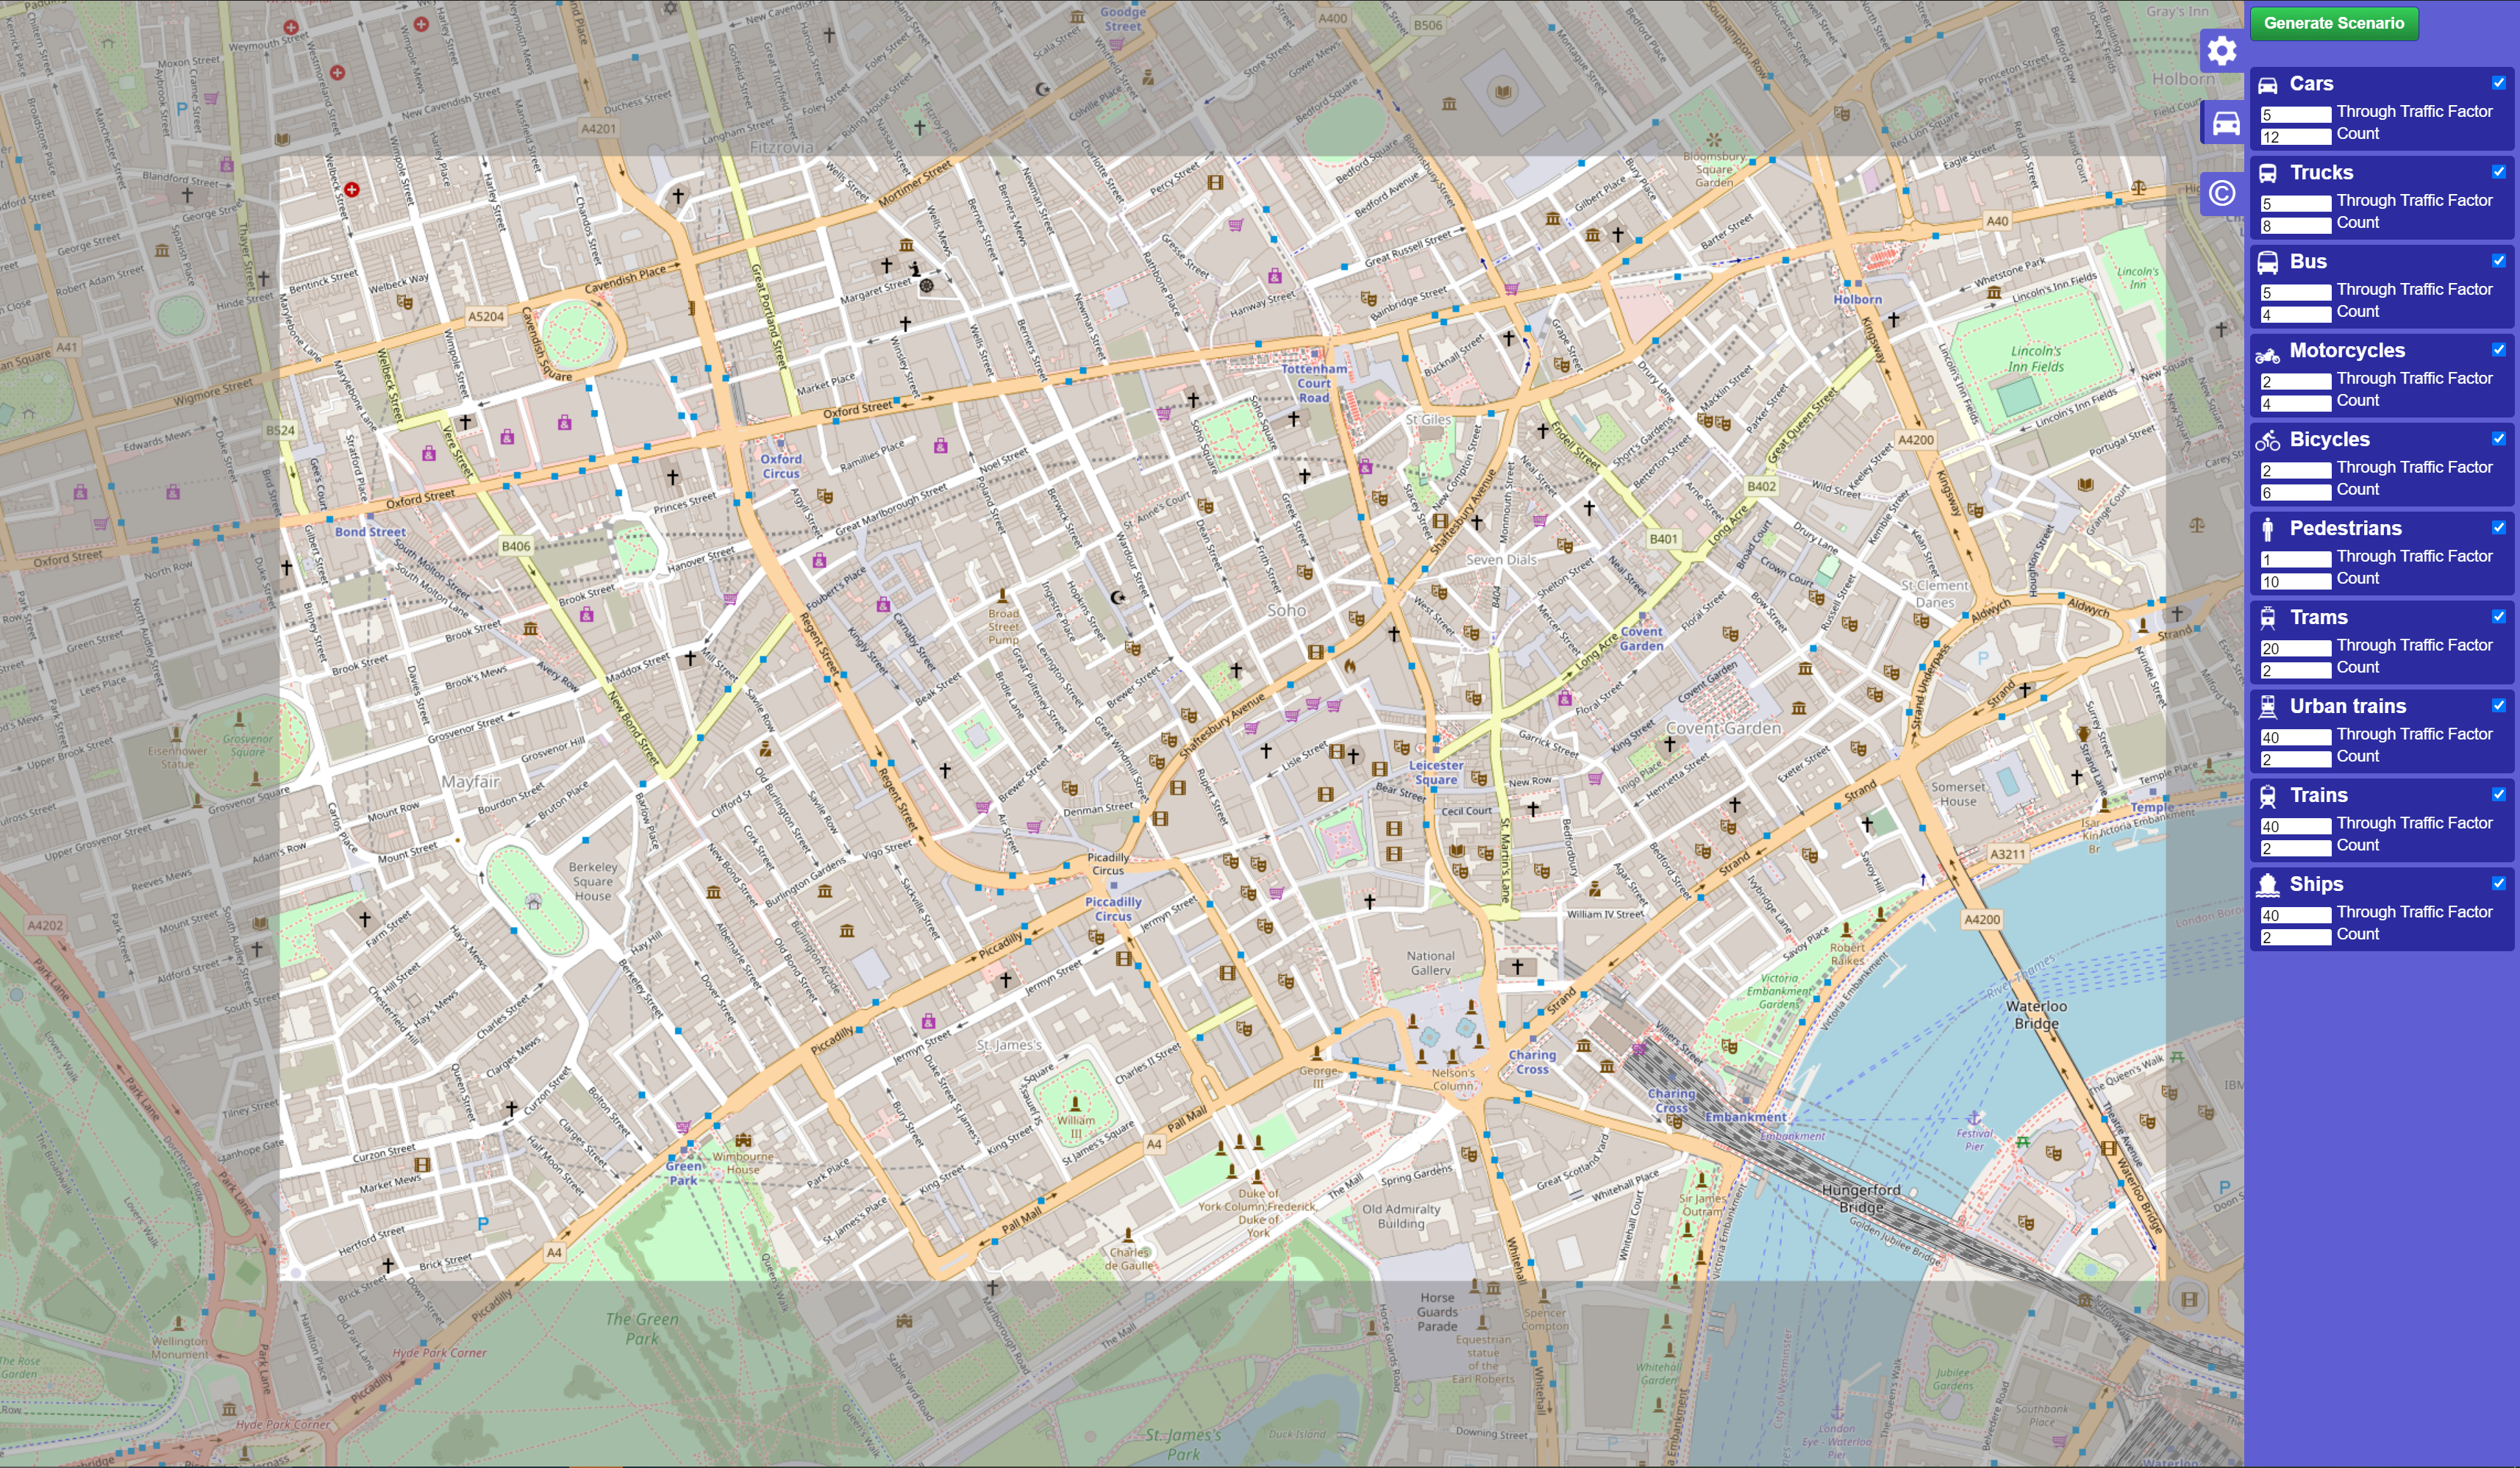
\includegraphics[width=1\linewidth]{osmWizard.PNG}
  \caption{\emph{OSMWebWizard} tool}
  \label{fig:7}
\end{figure}

\newpage

\subsection{Electric Vehicle and Charging Station Models}

As discussed above in the design chapter Section 3.5.1, \emph{SUMO} has an accurate EV and charging station model that mimics the real-world behaviours of both. For an EV after each time step of the \emph{SUMO} simulation, energy lost in that time step is subtracted from its current battery capacity. Attributes such as air density, vehicle front surface area, gravity acceleration, covered distance, rolling resistance coefficient, centripetal force, curve resistance coefficient and average power of constant consumers all contribute to the energy lost from the movement of the EV \autocite{kurczveil2013implementation}.

\begin{lstlisting}[language=Python, caption=Utility function to define EV model, label={lst:2}]
        f = open("data/electricvehicles.rou.xml", "r+")
        f.truncate(0)       # Clear file
    
        with open("data/electricvehicles.rou.xml", "w") as routes:
            sys.stdout = routes
            print("<routes>")
            print("""  <vType id="electricvehicle" accel="0.8" decel="4.5" sigma="0.5" emissionClass="Energy/unknown" minGap="2.5" maxSpeed="40" guiShape="evehicle" vClass="evehicle">
                         <param key="has.battery.device" value="true"/>
                         <param key="maximumBatteryCapacity" value="2000"/>
                         <param key="maximumPower" value="1000"/>
                         <param key="vehicleMass" value="1000"/>
                         <param key="frontSurfaceArea" value="5"/>
                         <param key="airDragCoefficient" value="0.6"/>
                         <param key="internalMomentOfInertia" value="0.01"/>
                         <param key="radialDragCoefficient" value="0.5"/>
                         <param key="rollDragCoefficient" value="0.01"/>
                         <param key="constantPowerIntake" value="100"/>
                         <param key="propulsionEfficiency" value="0.9"/>
                         <param key="recuperationEfficiency" value="0.9"/>
                         <param key="stoppingTreshold" value="0.1"/>
                 </vType>""")
            print("</routes>")
\end{lstlisting}

To implement EVs in \emph{SUMO} they first need to be defined \autocite{sumoElectric}. For this, a utility function was created which is illustrated in listing \ref{lst:2}. This dynamically defines the electric vehicle model for the simulation with all needed EV attributes.

Charging stations in simulation networks are surfaces on lanes that activate EV charging once the vehicle has driven over it. Attributes of a CS include the lane in which it resides, power output in wattage, charging efficiency, delay before vehicle starts to charge and whether it charges in transit so the vehicle does not have to stop. In a real-world scenario, plug-in charging stations are mostly deployed on parking bays where the vehicles park up and wait for them to charge. For our simulation we need to replicate this. Figure \ref{fig:8} shows how charging stations will be implemented on the networks. They will work as a bypass/parking bay which can be only accessed by the EV vehicle type in \emph{SUMO}.

\begin{figure}[h!]
  \centering
  \includegraphics[width=0.7\linewidth]{sumoCS.PNG}
  \caption{Charging station on a SUMO network}
  \label{fig:8}
\end{figure}

\subsection{TraCi Simulation Connection}

Once the \emph{SUMO} network is configured, the simulation can be initialised and connected to the \emph{Python} script using \emph{TraCi}. Listing \ref{lst:3} shows the commands to start the \emph{TraCi} simulation and the call to functionality for simulation control. Within the \emph{TraCi} start command outputs can be defined, "tripinfo-output" will give full information output on all vehicles in an XML file and "chargingstations-output" is all events that happened at each CS at each time step. The run function is where the \emph{TraCi} step loop is located which allows simulation manipulation and adjustment.

\begin{lstlisting}[language=Python, caption=TraCi simulation connection, label={lst:3}]
    traci.start([sumoBinary, "-c", "data/osm.sumocfg",
                             "--tripinfo-output", "tripinfo.xml", "--additional-files", "data/additionals.add.xml",
                             "--chargingstations-output", "data/chargingstations.xml"])
    main.run(netFile='data/osm.net.xml',
             additionalFile='data/additionals.add.xml',
             options=options)
\end{lstlisting}

\section{Algorithm Implementation}

After the \emph{SUMO} networks have been created, models integrated and the connection has been established with the \emph{Python} and \emph{TraCi} script, the algorithm can then be implemented. 

\subsection{Building a Graph}

To begin, a graph object needs to be created which will be populated with data from the \emph{SUMO} networks. The graph object will be used throughout the process of finding a detour for the EV. The \emph{SUMO} \emph{Python} module \emph{sumolib} provides methods that allow easy interaction with \emph{SUMO} network files and aids in retrieving information about the network. The graph objects properties include:

\begin{itemize}
  \item Net = The network XML file.
  \item Edges = All network edges.
  \item Nodes = All network nodes.
  \item Node Neighbours = All nodes that allow EVs, its neighbouring nodes, the connecting edge and its length.
  \item Charging Stations = All charging stations within the network.
  \item Max Speed = Max speed across the whole network.
  \item Connections = Internal lanes within in a junction.
\end{itemize}

\begin{lstlisting}[language=Python, caption=Graph Python object, label={lst:4}]
    class Graph:
        def __init__(self, netFile, additionalFile):
            self.Net = sumolib.net.readNet(netFile)
            self.Edges = self.Net.getEdges()
            self.Nodes = self.Net.getNodes()
            self.NodeNeighbours = self.getNodeNeighbours()
            self.ChargingStations = self.getChargingStations(additionalFile)
            self.MaxSpeed = self.getMaxSpeed(netFile)
            self.Connections = self.getConnections(netFile)
\end{lstlisting}

Listing \ref{lst:4} highlights the initialisation of the \emph{Graph} object in \emph{Python}. The function \emph{NodeNeighbours()} gets all nodes in the network that an electric vehicle can use with its neighbours, the edge that connects them and the length of that edge. Function \emph{ChargingStations()} gets all charging stations defined in the network, \emph{MaxSpeed()} gets the max speed across the whole network and \emph{getConnections()} gets all internal lane connections for accurate distance measurements. Internal lanes are the hidden lanes inside nodes (junctions) that vehicles follow when going from edge to edge.

\subsection{Routing Algorithm Outline}

The entry point of the routing algorithm is implemented next. Based on the design in Section 3.1, the function will be the initial call point and will hold the base functionality for the overall routing scheme. Listing \ref{lst:5} highlights the variable declarations at the beginning of the function. It begins with the conversion of the start and end edges to nodes. In \emph{SUMO} route assignment is done through edges but for calculating graph traversal nodes are needed. After this, the full battery capacity in kilowatt-hour for the EV being re-routed and the range in meters with the current capacity is found. Vehicle range is needed for routing calculations to make sure the EV will make the journey. The final variable assignment is the node from which charging stations will be searched from (\emph{csSearchNode}). Charging stations are searched for from a specific node due to longer routes with multiple stops, searches will be needed when range dips below the limit or more stops would be needed with fewer battery capacity gains.

\begin{lstlisting}[language=Python, caption=Routing initialisation function variable declarations, label={lst:5}]
    def rerouter(start, end, evID, graph):
        startNode = graph.Net.getEdge(start).getFromNode().getID()
        endNode = graph.Net.getEdge(end).getToNode().getID()
        evFullBatteryCapacity = float(traci.vehicle.getParameter(evID, 'device.battery.actualBatteryCapacity'))
        evRange = estimateRange(evFullBatteryCapacity)
        evRangeAtCS = evRange
        evRangeAtSearch = 0
    
        route = []
        routeLength = 0
        csStops = []
        csSearchNode = graph.Net.getEdge(start).getFromNode().getID()
\end{lstlisting}

Now that the variables are declared, the main routing loop can be initialised. Listing \ref{lst:6} below shows the while loop and functionality which gets the route and stops for the EV. The loop continues until the end node is reached or no routing solution can be found. It begins by finding an initial route for the EV from the start to the end nodes using the functionality defined in Section 4.2.4. If the last node in the route list is the end node then a route has successfully been found. The full route will be appended to the output route, duration needed at the last charging station calculated in the function \emph{'calculateCSRefuel()'} and the while loop broken. When the last node is not the end node, routing via a charging station begins. 

Section 4.2.5 highlights the implementation for the function \emph{'routeViaCS()'} which finds a route for the EV via a CS. Routing via a CS is first attempted with the CS search node being the location where range dropped below the threshold in the initial A* search, if no solution found the here the search node is then set to be equal to the start node. If no route again has not been found then there is no valid detour for the EV. When a detour has been found the route, route length and CS stop are all appended to the output variables. A new start node is also assigned as the node after the charging station where refuelling, allowing the next stage of the route to be calculated from the CS to the end. Finally, the duration at the CS stop is calculated to get 100\% state of charge(SoC) in function \emph{'calculateCSRefuel()'}. SoC is the current battery capacity relative to the actual battery capacity as a percentage from 0\% - 100\%. The assumption that charging will be done until 100\% SoC has been reached is due to not knowing the length of the next stage of the route, so accurate computation will be done when the end node is reached and the next stage of the route has been defined. The while loop is iterated until the end node is reached.

\begin{lstlisting}[language=Python, caption=Main iterator loop for routing solution, label={lst:6}]
    while True:
        tempRoute, tempLength = aStarSearch(startNode, endNode, evRange, False)

        # When initial route gets something back, saves route and sets new start as last node
        if tempRoute != []:
            csSearchNode = graph.Net.getEdge(tempRoute[-1]).getToNode().getID()
            evRangeAtSearch = evRange - tempLength

            # End cycle for route search if reached the end node
            if graph.Net.getEdge(tempRoute[-1]).getToNode().getID() == endNode:
                evRange, csStops = calculateCSRefuel(evRangeAtCS, csStops, tempLength, 10)
                route += tempRoute
                routeLength += tempLength
                break

        tempRoute, tempLength, csStop = routeViaCS(startNode, endNode, evRangeAtSearch, csSearchNode, evRange, hyperParams)

        if tempRoute == None:
            # Check if can route CS from start instead when no route from start node
            tempRoute, tempLength, csStop = routeViaCS(startNode, endNode, evRange, startNode, evRange, weightings)

            if tempRoute == None:
                print('No valid route for EV with current capacity')
                route = []
                routeLength = 0
                break

        route += tempRoute
        routeLength += tempLength

        # Set new start node from node after charging station
        # Used to find next section route
        startNode = graph.Net.getEdge(route[-1]).getToNode().getID()
        csStops.append(csStop)

        # Get current EV range that has just been travelled
        evRange -= tempLength
        evRangeAtCS -= tempLength

        # Set ev range as 100% making as can charge full at cs
        # Work out correct when get next route
        evRange, csStops = calculateCSRefuel(evRange, csStops, tempLength, 100)

\end{lstlisting}

Once the main loop has been broken, depending on if a route has been found or not, the route and charging station stops will be returned to the main \emph{TraCi} control loop to be assigned to the EV as shown in Section 4.2.7.

\subsection{EV Energy Calculations}

EV range calculations are needed for sufficiency checks of battery capacity when routing. These checks ensure the vehicle will make the journey with its current battery attributes. 

\begin{lstlisting}[language=Python, caption=Range estimation function, label={lst:7}]
    # Estimates range for EV from current battery capacity
    # Returns value in meters
    def estimateRange(batteryCapacity):
        return batteryCapacity * getMetersPerWatt(evID)
    
    # Estimate the battery capacity needed from refuel at charging station to get to destination
    # Returns value in Wh
    def estimateBatteryCapacity(evRange):
        return evRange / getMetersPerWatt(evID)
\end{lstlisting}

Listing \ref{lst:7} above estimates the remaining range of the EV and battery capacity. The range estimation takes in the current battery capacity in wattage and multiplies it by the meters per Watt-hour. The capacity estimation uses the EV range at the current time step of simulation and divides it by meters per Watt-hour.

\begin{equation} \label{eq:8}
    mWh=distanceDriven/totalEnergyConsumed
\end{equation}

Equation \ref{eq:8} illustrates how meters per Watt-hour(mWh) is calculated in \emph{SUMO}. Used in the range and battery capacity estimations, meters per Watt-hour is the energy used by the electric vehicle per meter. For \emph{SUMO} mWh needs to be computed by a previous simulation of the electric vehicle or by letting the vehicle run in a simulation for a few time steps due to needing distance driven and energy consumed over that distance which are found when running the simulation. After each time step the mWh for the EV will be recorded then at the end each are compared to find the mean and that will be the one used when calculating estimates. 

\begin{lstlisting}[language=Python, caption=Function to estimate State of Charge (SoC) of EV, label={lst:8}]
    def estimateSOC(evRange, routeLength):
        currentRange = evRange - routeLength
        currentSOC = (estimateBatteryCapacity(currentRange) / float(traci.vehicle.getParameter(evID, 'device.battery.maximumBatteryCapacity'))) * 100
        
        return currentSOC if currentSOC < 100 else 100
\end{lstlisting}

The final energy calculation is an estimation of the SoC of the EV which is shown in listing \ref{lst:8}. This is used throughout A* calculations when checking if battery capacity falls below the limit.

\subsection{A* Implementation}

As discussed in Section 3.2, the A* path-finding algorithm will be used in the solution for network (graph) traversal and finding the route. Our solutions A* implementation uses an open and closed list which stores all nodes that will be evaluated and all evaluated nodes. The open list, closed list, route, route cost and route length variables are all first declared at the beginning as shown in listing \ref{lst:9}. The open list is initialised with the start due to this being the first node that is going to be evaluated.

\begin{lstlisting}[language=Python, caption=Variable intialisations for A* search, label={lst:9}]
    openList = set([start])
    closedList = set([])

    route = {}
    route[start] = start

    routeCost = {}
    routeCost[start] = 0

    routeLength = {}
    routeLength[start] = 0
\end{lstlisting}

Finding a route requires iterations for node evaluation so a while loop is needed which will loop until the open list is empty, meaning no more nodes to evaluate. To start, the current node to be evaluated is set, which is found by looping through the open list and getting the value with the least routing cost as shown in \emph{Python} code listing \ref{lst:10}. Also, this is the first use of the heuristic function which uses the distance between the nodes dividing by max speed on the graph and will be a guide for the search so excess nodes do not need to be evaluated. 

\begin{lstlisting}[language=Python, caption=Choosing which node to evaluate next in A*, label={lst:10}]
    for node in openList:
            if currentNode == None \
                or routeCost[node] + heuristic(graph, node, end) < routeCost[currentNode] + heuristic(graph, currentNode, end):
                currentNode = node;
\end{lstlisting}

The next step is to implement stopping criteria for the search when certain constraints are met. As shown in the listing below, there are three different ways routing can be stopped at this stage. The first is when there is no current nodes being evaluated, this means the graph is empty or an error with the input of the start and end nodes. Next, checks are in place for when routing has reached the end node and A* has successfully completed searching, the route computed can then be output. Lastly, stopping is in place for when the EV range drops below the current SoC limit which is defaulted at 10. The route will then be outputted up to when the SoC dropped below the limit.

\begin{lstlisting}[language=Python, caption=Stopping criteria for A*, label={lst:11}]
    if currentNode == None:
        return None, 0

    if currentNode == end:
        return reconstructRoutePath(graph, start, currentNode, route, routeLength)

    # Checks whether soc under the limit when getting initial route or route from C

        if currentSOC < 11:
            return reconstructRoutePath(graph, start, currentNode, route, routeLength)
\end{lstlisting}

Lastly, the evaluation of node neighbours is done to add the best and least cost-effective neighbour nodes from the currently evaluated node, listing \ref{lst:12} illustrates this. It begins by checking if the current node has any neighbours, if not it means the node results in a dead-end and will not be evaluated. Each node is then evaluated, firstly checking if each node is in the open and closed lists and adding them to the open list and route if not. After this, if the node is in open and closed lists then checks are in place to see if it is quicker to visit the current node to the current neighbour node, again if so, then added to the route. Lastly, once all neighbours are evaluated the current node is added to the closed list, having already been evaluated and removed from the open list.

\begin{lstlisting}[language=Python, caption=A* neighbouring nodes evaluation, label={lst:12}]
    # Checker to not evaluate nodes that lead to dead end
    if graph.neighbors(currentNode) != None:
        for next in graph.neighbors(currentNode):
            neighbourNode = next['Neighbour']
            edgeStepSpeed = traci.edge.getLastStepMeanSpeed(next['ConnectingEdge'])

            if neighbourNode not in openList and neighbourNode not in closedList:
                openList.add(neighbourNode)
                route[neighbourNode] = currentNode

                # Travel time is cost of each node, length / speed of road, this gets fastest and shortest route
                routeCost[neighbourNode] = routeCost[currentNode] + (next['Length'] / edgeStepSpeed)
                routeLength[neighbourNode] = routeLength[currentNode] + next['Length']

            else:
                if routeCost[neighbourNode] > routeCost[currentNode] + (next['Length'] / edgeStepSpeed):
                    routeCost[neighbourNode] = routeCost[currentNode] + (next['Length'] / edgeStepSpeed)
                    route[neighbourNode] = currentNode
                    routeLength[neighbourNode] = routeLength[currentNode] + next['Length']

                    if neighbourNode in closedList:
                        closedList.remove(neighbourNode)
                        openList.add(neighbourNode)

    closedList.add(currentNode)
    openList.remove(currentNode)
\end{lstlisting}

\subsection{Selecting a Charging Station}

Once the EV range is insufficient, the selection of a charging station on the route is needed. Listing \ref{lst:13} highlights the function called when routing via a charging station.

\begin{lstlisting}[language=Python, caption=Initial call to route via a CS, label={lst:13}]
    def routeViaCS(startNode, endNode, evRangeAtSearch, csSearchNode, evRange, hyperParams):
        closestCSs = getNeighbouringCS(csSearchNode, endNode, evRangeAtSearch)
    
        if len(closestCSs) > 0:
            chargingStation = getBestCS(closestCSs, hyperParams)
            csStartNode = graph.Net.getEdge(chargingStation.Lane).getFromNode().getID()
    
            route, routeLength = aStarSearch(startNode, csStartNode, evRange, True)
    
            if route == None:
                return None, None, None
    
            # Append the connecting node to the edge where the CS
            # lies incase more than one edge coming from start node
            routeLength += graph.Net.getEdge(chargingStation.Lane).getLength()
            route.append(chargingStation.Lane)
    
            return route, routeLength, chargingStation
    
        print('Error, no charging stations available for EV.')
        return None, None, None
\end{lstlisting}
 
Firstly, all charging stations in the vicinity of the range of the vehicle are found in \emph{getNeighbouringCS} and properties relating to selection using SAW are found. Initially, the neighbouring CSs from the vicinity of the CS search node are found using vehicle range at that node. If no CSs are found then no routing can be done for EV with current battery capacity. 

Listing \ref{lst:14} below highlights the functionality within the \emph{getNeighbouringCS} function. Checking the charging station is within the radius of the EV range is done by using the Pythagoras theorem to get the distance between current and charging station locations then checking if the value is less than the radius. After CS is found to be within the vicinity then the properties used within SAW are found such as \emph{DistanceFromStart}, \emph{DistanceFromDivider}, \emph{VehiclesCharging} and \emph{price}. The \emph{DistanceFromStart} is the euclidean distance from the current EV location to the CS location and \emph{DistanceFromDivider} is the distance from the divider drew from the start to the endpoint, which gets the direction the CS is in. The \emph{VehiclesCharging} attribute is found by running the \emph{traci} command \emph{'getVehicleCount'} listed below which gets the total number of vehicles stopped and waiting at the CS.

\begin{lstlisting}[language=Python, caption=Functionality for getting neighbouring CSs, label={lst:14}]
    lineDistance = euclideanDistance(nodeCoords, endCoords)
    chargingStations = []

    for cs in graph.ChargingStations:
        if checkCSInRadius(nodeCoords, cs.X, cs.Y, radius):
            cs.DistanceFromStart = euclideanDistance(nodeCoords, [cs.X, cs.Y])
            cs.DistanceFromDivider = distanceFromLine(nodeCoords, endCoords, [cs.X, cs.Y], lineDistance)
            cs.VehiclesCharging = traci.chargingstation.getVehicleCount(cs.id)
            cs.Price = uniform(0.1, 0.25)

            chargingStations.append(cs)
\end{lstlisting}

Once all available CSs are found the optimal one can then be chosen based on SAW and the weightings defined. The \emph{getBestCS} function shown in the listing below displays the implementation of SAW. Using the formulas denoted in Section 3.3.1, each attribute is normalized using vector normalization, then multiplied by their given weighting and each value added together to get an overall score. The CS with the highest score is then outputted as the best one to route via.

\begin{lstlisting}[language=Python, caption=Python function that uses SAW to find best CS, label={lst:15}]
    def getBestCS(closestCSs, weightings):
        # Get vector lengths for denomatonator for all attributes
        lenDistStart = math.sqrt(sum(cs.DistanceFromStart ** 2 for cs in closestCSs))
        lenDistDivider = math.sqrt(sum(cs.DistanceFromDivider ** 2 for cs in closestCSs))
        lenPrice = math.sqrt(sum(cs.Price ** 2 for cs in closestCSs))
        lenVehiclesCharging = math.sqrt(sum(cs.VehiclesCharging ** 2 for cs in closestCSs))
        lenStepCharge = math.sqrt(sum(cs.ChargePerStep ** 2 for cs in closestCSs))
    
        for cs in closestCSs:
            # Normalize each attribute of CS wish to make decision based on and  its weighting
            distStartScore = (1 - (cs.DistanceFromStart / lenDistStart)) * weightings["DistanceFromStart"]
            distDividerScore = (1 - (cs.DistanceFromDivider / lenDistDivider)) * weightings["DistanceFromDivider"]
            priceScore = (1 - (cs.Price / lenPrice)) * weightings["Price"]
            vehiclesChargingScore = (1 - (cs.VehiclesCharging / lenVehiclesCharging)) * weightings["VehiclesCharging"]
            stepChargeScore = (cs.ChargePerStep / lenStepCharge) * weightings["ChargePerStep"]
    
            # Get CS score of best charging station
            cs.Score = distStartScore + distDividerScore + priceScore + stepChargeScore + vehiclesChargingScore

        return max(closestCSs, key=lambda item: item.Score)
\end{lstlisting}

Finally, drawing back to listing \ref{lst:13}, once the best charging station has been found, a route from the current node to the CS will be constructed using the functionality described in Section 4.2.4 and returned to be appended to the overall route. If no route is found again or the function outputs \emph{None} types for the route and route lengths, the EV does not have a valid solution for its current attributes.

\subsection{Calculating Charging Station Refuel}

Once the route has been found and there is a CS stop on the route, a function is needed to compute the stopping duration at the charging station. The duration taken at a charging station affects the amount of charge an EV will gain. 

\begin{lstlisting}[language=Python, caption=Function to compute CS refuel time, label={lst:16}]
    # Get the correct range and duration needed from and for EV for last charging station stop
    def calculateCSRefuel(evRange, chargingStations, routeLength, goalPercentage):
        if len(chargingStations) > 0:
            # Get meters still needed to travel to complete journey
            rangeNeeded = routeLength - evRange
            currentEstCapacity = estimateBatteryCapacity(evRange)
            maxBatteryCapacity = float(traci.vehicle.getParameter(evID, 'device.battery.maximumBatteryCapacity'))
    
            capacityNeeded = (estimateBatteryCapacity(rangeNeeded)) + (maxBatteryCapacity * 0.1)
            capacityGoal = maxBatteryCapacity * (goalPercentage / 100)
    
            # Needed capacity as max battery capacity if greater
            # Ensure no unnecessary time wasted at CS
            if capacityNeeded > maxBatteryCapacity:
                capacityNeeded = maxBatteryCapacity - currentEstCapacity
    
            # Goal capacity as max battery capacity if goal greater
            # Ensure no unnecessary time wasted at CS
            if capacityGoal > maxBatteryCapacity:
                capacityGoal = maxBatteryCapacity - currentEstCapacity
    
            csChargePerStep = (chargingStations[-1].Power * chargingStations[-1].Efficiency) / 3600
            durationToNeeded = math.ceil(capacityNeeded / csChargePerStep)
            durationToGoal = math.ceil(capacityGoal / csChargePerStep)
    
            # Get higher duration of two for time spent charging at CS
            chargingStations[-1].Duration = max(durationToNeeded, durationToGoal)
            newCapacity = currentEstCapacity + (chargingStations[-1].Duration * csChargePerStep)
    
            evRange = estimateRange(newCapacity)
            evRange -= routeLength
    
        return evRange, chargingStations
\end{lstlisting}

The above \emph{Python} code illustrates how charging station stopping duration is computed. Firstly, the function checks there is a CS stop within the route. When there is, capacity needed for the rest of the route from the CS is calculated from the current and maximum EV battery capacities. As well as capacity needed, a capacity goal is set out which calculates a goal battery capacity that the CS has to be over after recharging. Now, the EV charge gained in Kw per step has to be calculated so computation can be done to find the duration it will take to reach both capacity needed and capacity goal. Below shows the formula used to get the charge per step of a charging station.
\begin{equation} \label{eq:9}
    cPs=(csPower*csEfficiency)/3600 
\end{equation}
With both duration's now found for the needed and goal capacities, the max out of the two is assigned to the charging station because the higher value will ensure both capacity goal and needed will be met. Lastly, the new battery capacity and EV range are estimated to ensure the next time route searching is done it has the correct values and no inaccuracies with EV battery checks.

\subsection{Routing SUMO Electric vehicle}

Finally, the last step of the detour computation scheme is assigning the new route and charging station stops to the simulated vehicle. The below listing shows how to assign vehicle route and CS stops using \emph{TraCi}. Once a valid route and stops are found they are both appointed to the vehicle. Charging station stops are set using their \emph{SUMO} network ID and the time step duration in which the vehicle will be stopping for.

\begin{lstlisting}[language=Python, caption=Functionality to assign new route and CS stops, label={lst:17}]
    route, csStops = rerouter(startNode, endNode, vehicleID, graph)

    if len(route) > 0:
        traci.vehicle.setRoute(vehicleID, route)

        for chargingStation in csStops:
            traci.vehicle.setChargingStationStop(vehicleID, chargingStation.id, duration=chargingStation.Duration)
\end{lstlisting}

\section{Conclusion}

Overall, this chapter illustrates how the detour computation scheme was implemented into a \emph{SUMO} simulation of a real-world transport network with detailed explanation of how ideas from the design were carried out.

\newpage 

\chapter{Performance Evaluation}

\newpage

\chapter{Conclusion and Future Works}

\newpage

\newpage

\printbibliography

\newpage

\listoffigures

\newpage

\listoftables

\newpage

\lstlistoflistings

\end{document}